%%%%%%%%%%%%%%%%%%%%%%%%%%%%%%%%%%%%%%%%%%%%%%%%%%%%%%%%%%%%%%%%%%%%%%%%%%%%%%%%
%2345678901234567890123456789012345678901234567890123456789012345678901234567890
%        1         2         3         4         5         6         7         8

\documentclass[letterpaper, 10 pt, conference]{ieeeconf}  % Comment this line out
                                                          % if you need a4paper
%\documentclass[a4paper, 10pt, conference]{ieeeconf}      % Use this line for a4
                                                          % paper

\IEEEoverridecommandlockouts                              % This command is only
                                                          % needed if you want to
                                                          % use the \thanks command
\overrideIEEEmargins
% See the \addtolength command later in the file to balance the column lengths
% on the last page of the document

\usepackage[utf8]{inputenc}
\usepackage[T1]{fontenc}
\usepackage[utf8]{inputenc}
\usepackage[T1]{fontenc}
\usepackage{float}
\usepackage{graphicx}
\usepackage{cite}
\usepackage{amsmath,amssymb,amsfonts}
\usepackage{graphicx,color}
\usepackage{listings}
\usepackage{xcolor}
\usepackage{algorithm}
\usepackage{algpseudocode}
\usepackage{float}
\usepackage{placeins}
% Optional: Styling for Python code to look professional
\definecolor{codegreen}{rgb}{0,0.6,0}
\definecolor{codegray}{rgb}{0.5,0.5,0.5}
\definecolor{codepurple}{rgb}{0.58,0,0.82}
\definecolor{backcolour}{rgb}{0.95,0.95,0.92}

\lstdefinestyle{mystyle}{
    backgroundcolor=\color{backcolour},   
    commentstyle=\color{codegreen},
    keywordstyle=\color{magenta},
    numberstyle=\tiny\color{codegray},
    stringstyle=\color{codepurple},
    basicstyle=\ttfamily\footnotesize,
    breakatwhitespace=false,         
    breaklines=true,                 
    captionpos=b,                    
    keepspaces=true,                 
    numbers=left,                    
    numbersep=5pt,                  
    showspaces=false,                
    showstringspaces=false,
    showtabs=false,                  
    tabsize=2
}

\lstset{style=mystyle}



% The following packages can be found on http:\\www.ctan.org
%\usepackage{graphics} % for pdf, bitmapped graphics files
%\usepackage{epsfig} % for postscript graphics files
%\usepackage{mathptmx} % assumes new font selection scheme installed
%\usepackage{mathptmx} % assumes new font selection scheme installed
%\usepackage{amsmath} % assumes amsmath package installed
%\usepackage{amssymb}  % assumes amsmath package installed

\title{\LARGE \bf
An Intelligent System for Sleep Disorder Detection and Lifestyle Recommendation Using Polysomnography Data
}

%\author{ \parbox{3 in}{\centering Huibert Kwakernaak*
%         \thanks{*Use the $\backslash$thanks command to put information here}\\
%         Faculty of Electrical Engineering, Mathematics and Computer Science\\
%         University of Twente\\
%         7500 AE Enschede, The Netherlands\\
%         {\tt\small h.kwakernaak@autsubmit.com}}
%         \hspace*{ 0.5 in}
%         \parbox{3 in}{ \centering Pradeep Misra**
%         \thanks{**The footnote marks may be inserted manually}\\
%        Department of Electrical Engineering \\
%         Wright State University\\
%         Dayton, OH 45435, USA\\
%         {\tt\small pmisra@cs.wright.edu}}
%}

\author{Girish S (AM.EN.U4AIE22044), Harishankar Binu Nair (AM.EN.U4AIE22023)}


\begin{document}



\maketitle
\thispagestyle{empty}
\pagestyle{empty}


%%%%%%%%%%%%%%%%%%%%%%%%%%%%%%%%%%%%%%%%%%%%%%%%%%%%%%%%%%%%%%%%%%%%%%%%%%%%%%%%
\begin{abstract}
Sleep disorders such as insomnia, sleep apnea, and restless leg syndrome affect millions worldwide and pose a growing public health challenge. In developing regions such as India, limited access to sleep clinics, social stigma, and low awareness contribute to significant under diagnosis, delaying effective intervention and management. Current diagnostic practices rely on in-laboratory polysomnography and expert interpretation, which are expensive, resource-intensive, and unsuitable for population-scale screening. Although recent artificial intelligence based approaches have shown promise in automating sleep stage analysis, many existing systems lack clinical interpretability and fail to translate model outputs into actionable guidance for patients. To address these limitations, this work proposes an interpretable and automated sleep disorder detection framework with limited channel selected to improve data collection process for the users. Mainly, this work attempts to tackle challenges such as data collection reproducibility, interpretable results, cloud deployable model for sleep staging. This project provides a implementation of a custom sleep staging architecture with self attention mechanism to produce interpretable heat-maps and specifically designed for light weight deployment in cloud environment reducing inference latency. By combining automated analysis, clinical interpretability, and interactive patient education within a single platform, the proposed solution enables early screening, improves sleep health awareness, and supports scalable deployment in low-resource settings. The system is designed to bridge the gap between clinical expertise and public usability, offering a transparent, privacy-conscious, and accessible approach to sleep disorder assessment and management. 
\end{abstract}


%%%%%%%%%%%%%%%%%%%%%%%%%%%%%%%%%%%%%%%%%%%%%%%%%%%%%%%%%%%%%%%%%%%%%%%%%%%%%%%%
\section{Introduction}
\label{sec:introduction}

Sleep is a fundamental biological process that plays a critical role in physical restoration, cognitive functioning, emotional regulation, immune response, and metabolic homeostasis. Adequate and well-structured sleep is essential for memory consolidation, emotional resilience, cardiovascular regulation, and overall quality of life. The sleep-wake cycle is regulated by complex interactions between circadian rhythms, homeostatic sleep pressure, and neurochemical processes involving multiple brain regions, including the suprachiasmatic nucleus, brainstem, and thalamocortical networks. During sleep, the body undergoes essential restorative processes including tissue repair, protein synthesis, immune system modulation, and clearance of metabolic waste products from the central nervous system. These processes are critical for maintaining optimal physiological function and preventing the accumulation of pathological changes that can lead to chronic disease states.

Persistent disturbances in sleep duration, continuity, timing, or architecture give rise to sleep disorders, a heterogeneous group of conditions that significantly impair daily functioning and increase long-term health risks~\cite{icsd2014}. Sleep disorders manifest through diverse mechanisms, including disruptions in sleep initiation, maintenance, or quality; abnormal sleep-related behaviors; breathing irregularities during sleep; and misalignments between internal circadian rhythms and external environmental cues. The clinical presentation of sleep disorders varies widely, ranging from subtle symptoms that may be dismissed as lifestyle issues to severe conditions that substantially compromise physical health, mental well-being, and social functioning. In recent decades, sleep disorders have emerged as a major global public health concern, affecting individuals across age groups, socioeconomic strata, and geographic regions, with consequences that extend beyond individual health to societal productivity and healthcare systems. The recognition of sleep disorders as a significant public health issue has been driven by accumulating epidemiological evidence linking sleep disturbances to increased morbidity, mortality, healthcare utilization, and economic burden.

Global epidemiological evidence suggests that sleep disturbances are alarmingly prevalent and represent one of the most common health complaints in clinical practice. Approximately 30–45\% of adults experience at least one form of sleep disturbance during their lifetime, while 10–30\% suffer from chronic insomnia symptoms~\cite{ohayon2002epidemiology,jehan2017insomniaglobal}. These figures likely represent conservative estimates, as many individuals with sleep problems do not seek medical attention or may not recognize their symptoms as indicative of a sleep disorder. The prevalence of sleep disturbances increases with age, with older adults experiencing higher rates of sleep fragmentation, reduced sleep efficiency, and increased prevalence of sleep-disordered breathing. Gender differences are also notable, with women reporting higher rates of insomnia but lower rates of obstructive sleep apnea compared to men, though these patterns may be influenced by hormonal factors, reporting biases, and diagnostic practices.

Obstructive sleep apnea (OSA), one of the most common yet underdiagnosed sleep-related breathing disorders, affects an estimated 3–7\% of adults, with higher prevalence among males, older populations, and individuals with obesity~\cite{peppard2013osaprevalence,senaratna2017osaprevalence,young1993osaprevalence}. More recent population-scale studies have reported OSA prevalence ranging from 9\% to 38\%, depending on diagnostic thresholds, screening criteria, and demographic characteristics~\cite{heinzer2015sleepapnea,lechat2021sleepapnea}. The wide variation in reported prevalence reflects differences in study methodologies, diagnostic criteria, population characteristics, and the evolving understanding of OSA severity thresholds. Importantly, a substantial proportion of individuals with moderate to severe OSA remain undiagnosed, with estimates suggesting that up to 80\% of cases may go unrecognized, particularly in populations with limited access to sleep medicine services. This underdiagnosis represents a significant missed opportunity for intervention, as untreated OSA is associated with increased cardiovascular risk, metabolic dysfunction, and impaired quality of life.

Movement-related sleep disorders, including restless legs syndrome and periodic limb movement disorder, affect an estimated 2–15\% of the general population, with prevalence increasing with age. Parasomnias, encompassing conditions such as sleepwalking, night terrors, and REM sleep behavior disorder, are less common but can have significant safety implications and quality of life impacts. Circadian rhythm sleep-wake disorders, including delayed sleep phase syndrome and shift work disorder, are increasingly recognized as contributors to the sleep disorder burden, particularly in modern societies with 24-hour operations and increased use of artificial lighting and electronic devices. These conditions further contribute to the disease burden, particularly among ageing populations, shift workers, and individuals with irregular schedules.

In the Indian context, community-based surveys and hospital-based studies indicate similarly high prevalence rates of sleep disorders~\cite{gupta2017indiasleep,chattu2019indiasleep}. Population-based studies from various regions of India have reported insomnia prevalence ranging from 10\% to 30\%, with higher rates observed in urban populations, women, and older adults. OSA prevalence in Indian populations has been estimated at 2–4\% in community samples, though this may represent significant underdiagnosis given the limited availability of diagnostic facilities. The burden of sleep disorders in India is compounded by several unique challenges. The country faces a critical shortage of sleep medicine specialists, with most sleep clinics concentrated in major metropolitan areas, leaving vast rural and semi-urban populations with limited or no access to specialized care. The cost of polysomnography, which can range from several thousand to tens of thousands of Indian rupees, places it beyond the reach of many individuals, particularly those from lower socioeconomic backgrounds who may be at higher risk for sleep disorders due to occupational hazards, environmental factors, and limited access to healthcare.

However, a substantial proportion of cases remain undiagnosed or untreated due to limited access to specialised sleep clinics, high diagnostic costs, uneven distribution of trained sleep professionals, and low public awareness. Social stigma surrounding sleep disorders, particularly when they are perceived as mental health issues or signs of laziness, further compounds the problem. Cultural factors, including traditional beliefs about sleep and health, may also influence help-seeking behavior. Lack of education regarding sleep health, misconceptions about sleep disorders as lifestyle choices rather than medical conditions, and limited integration of sleep medicine into primary healthcare systems further delay help-seeking behaviour, exacerbating the public health impact. The consequences of untreated sleep disorders in India are particularly concerning given the country's high burden of non-communicable diseases, including cardiovascular disease, diabetes, and mental health disorders, all of which are exacerbated by poor sleep quality.

The increasing prevalence of sleep disorders is closely linked to modern lifestyle and environmental factors that have fundamentally altered human sleep patterns over recent decades. Prolonged exposure to mobile devices and artificial light, particularly blue light emitted from screens, suppresses melatonin production and disrupts circadian phase alignment, leading to delayed sleep onset and reduced sleep quality. Excessive caffeine consumption, often used as a compensatory mechanism for sleepiness, creates a vicious cycle of sleep disruption and stimulant dependence. Irregular work schedules, including shift work and night shifts, directly conflict with natural circadian rhythms and have been associated with increased risk of sleep disorders, metabolic dysfunction, and cardiovascular disease. Chronic psychosocial stress, driven by work demands, financial pressures, and social obligations, activates the hypothalamic-pituitary-adrenal axis and sympathetic nervous system, promoting hyperarousal and sleep fragmentation. Reduced physical activity, sedentary lifestyles, and limited exposure to natural daylight further compromise sleep-wake regulation. Urban noise pollution, including traffic, construction, and industrial sounds, disrupts sleep continuity and prevents deep sleep stages, even when individuals do not consciously awaken.

These factors disrupt circadian rhythms and sleep homeostasis, leading to both acute sleep disturbances and chronic sleep pathology. The cumulative effect of these modern lifestyle factors has been described as contributing to a "sleep crisis" in contemporary society, with implications for individual health, workplace productivity, and public safety. When left untreated, sleep disorders are associated with a wide range of adverse health outcomes. Cardiovascular disease represents one of the most well-established consequences of sleep disorders~\cite{strollo2016cardiovascular,peppard2000longitudinal}, with OSA in particular being recognized as an independent risk factor for hypertension, coronary artery disease, stroke, and cardiac arrhythmias. The mechanisms linking sleep disorders to cardiovascular disease include intermittent hypoxia, sympathetic activation, endothelial dysfunction, and systemic inflammation. Metabolic consequences include insulin resistance, impaired glucose regulation, dyslipidemia, and increased risk of type 2 diabetes, with sleep restriction and fragmentation disrupting hormonal regulation of appetite and metabolism. The relationship between sleep disorders and mental health is bidirectional and complex, with depression and anxiety disorders both contributing to and resulting from sleep disturbances~\cite{baglioni2011depression}. Cognitive consequences include impaired attention, memory consolidation, executive function, and decision-making, with chronic sleep restriction leading to cumulative cognitive deficits that may not be fully reversible. Reduced work productivity, increased absenteeism, and presenteeism represent significant economic consequences, while the increased risk of occupational and road traffic accidents poses serious public safety concerns. Emerging evidence also highlights a bidirectional relationship between sleep disorders and inflammatory processes, further amplifying cardiometabolic and neuropsychiatric risks~\cite{irwin2019comorbidities}. Sleep disruption activates inflammatory pathways, while inflammatory conditions can disrupt sleep, creating a self-perpetuating cycle that contributes to disease progression.

\subsection{Scope}

Despite the growing burden of sleep disorders, accurate and timely diagnosis remains challenging due to the complexity of sleep physiology, the subjective nature of many sleep complaints, and the resource-intensive nature of comprehensive sleep evaluation. Overnight polysomnography (PSG) is widely regarded as the clinical gold standard for sleep disorder assessment~\cite{kapur2017clinical}. PSG provides comprehensive multimodal recordings of brain activity through electroencephalography (EEG), eye movements via electrooculography (EOG), muscle tone through electromyography (EMG), respiratory effort and airflow, oxygen saturation via pulse oximetry, and cardiac activity through electrocardiography (ECG). This comprehensive monitoring enables detailed analysis of sleep stages, respiratory events, limb movements, arousals, and other physiological phenomena that are essential for accurate diagnosis.

However, PSG analysis relies heavily on manual sleep stage scoring and expert interpretation, processes that are time-consuming, resource-intensive, and subject to inter- and intra-scorer variability. Manual sleep stage scoring requires trained technicians to visually inspect 30-second epochs of EEG, EOG, and EMG signals, applying standardized criteria to classify each epoch into wake, N1, N2, N3, or REM sleep stages. This process typically takes 2–4 hours for a single overnight recording, creating a significant bottleneck in sleep laboratories. Inter-scorer agreement, while generally good for clear cases, can vary substantially for transitional epochs and ambiguous patterns, with reported agreement rates ranging from 70\% to 90\% depending on the sleep stage and scorer experience. The identification of respiratory events, limb movements, and arousals requires additional expertise and time, further extending the analysis duration. The subjective nature of manual scoring introduces variability that can affect diagnostic accuracy and treatment decisions, particularly for borderline cases or when multiple scorers are involved in the same study.

These limitations significantly restrict scalability and delay diagnosis, particularly in low-resource healthcare settings where access to specialised sleep laboratories and trained professionals is limited. The high cost of PSG equipment, the need for dedicated sleep laboratory facilities, and the requirement for trained technicians create barriers to widespread implementation. Wait times for PSG studies can extend to several months in many regions, delaying diagnosis and treatment initiation. The inconvenience of overnight laboratory studies, including the need for patients to sleep in an unfamiliar environment, can also affect sleep quality and potentially influence study results. Although portable sleep monitoring systems and wearable devices have improved accessibility~\cite{aziz2025wearable}, they typically capture a limited subset of physiological signals and often lack robust analytical frameworks capable of reliable disorder detection~\cite{wongsirichot2017minimal}. Home sleep apnea testing devices, while more convenient and cost-effective than laboratory PSG, generally focus on respiratory parameters and may miss other sleep disorders or provide incomplete information for comprehensive sleep evaluation. Consequently, there is a critical need for automated, scalable, and interpretable systems that can effectively leverage PSG data while supporting both clinical decision-making and patient understanding. Such systems must maintain diagnostic accuracy while reducing the time and expertise required for analysis, enabling broader access to high-quality sleep disorder assessment.

\begin{figure*}
    \centering
    \includegraphics[width=1\linewidth]{overview_p2.png}
    \caption{Overview of the proposed system that integrates transformer-based sleep stage classification, explainable AI for clinical interpretability, and retrieval-augmented patient guidance to enable scalable, transparent, and accessible sleep health assessment.}
    \label{fig:DFD}
\end{figure*}

\subsection{Motivation}

Recent advances in artificial intelligence have demonstrated strong potential for automating sleep staging and sleep disorder detection using machine learning and deep learning models~\cite{xu2022deep}. Early approaches employed traditional machine learning techniques, including support vector machines, random forests, and k-nearest neighbors, applied to handcrafted features extracted from PSG signals. While these methods achieved reasonable performance, they required extensive domain expertise for feature engineering and were limited in their ability to capture complex temporal patterns and non-linear relationships in sleep data. The advent of deep learning has revolutionized automated sleep analysis, with convolutional neural networks (CNNs) enabling automatic feature extraction from raw or minimally processed signals, and recurrent neural networks (RNNs) and long short-term memory (LSTM) networks capturing temporal dependencies across sleep epochs.

In particular, transformer-based architectures have shown superior capability in modelling long-range temporal dependencies in multichannel PSG signals, achieving performance comparable to expert scorers in several benchmarks~\cite{chen2022joint}. These models are well-suited for capturing the hierarchical and sequential nature of sleep architecture, where the classification of a given epoch depends not only on its immediate characteristics but also on the broader context of the sleep episode, including preceding stages, sleep architecture patterns, and circadian influences. The attention mechanisms in transformer models allow them to selectively focus on relevant temporal segments and signal features, mimicking the way expert scorers integrate information across multiple channels and time points. Multi-task learning approaches that simultaneously perform sleep staging and disorder detection have shown promise in improving both tasks by leveraging shared representations and complementary information.

However, most existing AI-based systems operate as black boxes, providing predictions without transparent explanations, which limits clinical trust and impedes real-world adoption~\cite{xu2022deep}. Clinicians require understanding of the reasoning behind AI predictions to integrate them into clinical decision-making, particularly when recommendations may have significant implications for patient care. The lack of interpretability also hinders model validation, error analysis, and continuous improvement. Moreover, current solutions largely focus on diagnosis alone, offering little in terms of patient-centric guidance, education, or actionable recommendations. Patients often receive diagnostic labels without understanding what they mean, why they occurred, or what they can do to improve their sleep health. Given the strong influence of lifestyle and behavioural factors on sleep health, there is an increasing demand for intelligent systems that not only automate diagnosis but also deliver interpretable insights and personalised lifestyle recommendations, particularly in populations with limited access to sleep specialists. Such systems must bridge the gap between technical AI capabilities and practical clinical and patient needs, providing not just accurate predictions but also meaningful explanations and actionable guidance.

\subsection{Sleep Stages and Their Clinical Significance}

Sleep is organised into distinct stages defined by characteristic physiological patterns, as standardised by the American Academy of Sleep Medicine~\cite{berry2012aasm,berry2020aasm}. These stages reflect underlying neural and autonomic processes and serve as critical indicators of sleep quality and pathology. The current AASM scoring framework builds upon the foundational work of Rechtschaffen and Kales~\cite{rechtschaffen1968scoring}, establishing widely accepted criteria for sleep stage classification.

Sleep is broadly divided into wakefulness (W), non-rapid eye movement (NREM) sleep, and rapid eye movement (REM) sleep. NREM sleep is further subdivided into stages N1, N2, and N3, representing increasing depth of sleep. N1 corresponds to the transition from wakefulness to sleep, N2 is characterised by sleep spindles and K-complexes associated with memory processing and sensory gating, and N3 represents slow-wave sleep linked to physical restoration and metabolic regulation. REM sleep is associated with vivid dreaming, emotional regulation, and memory consolidation.

Alterations in sleep stage proportions, transitions, and continuity are strongly associated with specific sleep disorders. Fragmented sleep architecture and reduced slow-wave sleep are commonly observed in insomnia, while abnormal REM onset and instability are indicative of narcolepsy~\cite{wilaiprasitporn2017hypnodensity,chen2022joint}. Recurrent arousals and disrupted NREM–REM transitions are hallmark features of sleep-disordered breathing and movement-related disorders~\cite{alattar2024cap}.

Sleep disorders encompass a wide range of conditions with distinct physiological signatures, systematically classified in the International Classification of Sleep Disorders (ICSD-3)~\cite{icsd2014}. Major categories relevant to PSG-based diagnosis include insomnia, obstructive sleep apnea, restless legs syndrome and periodic limb movement disorder, narcolepsy, REM sleep behaviour disorder, and circadian rhythm sleep–wake disorders. Accurate identification of these conditions requires integrated analysis of sleep stages, physiological events, and temporal patterns across the entire PSG recording.

Although numerous AI-based methods for sleep analysis have been proposed~\cite{xu2022deep,wadichar2023two,urtnasan2021sleep}, several challenges remain unresolved. Many studies focus on isolated tasks such as sleep staging or single-disorder detection~\cite{urtnasan2022plmd}, limiting clinical applicability. Models often lack interpretability, hindering clinician trust, while patient-centric explanations and actionable guidance are rarely addressed~\cite{aziz2025wearable}. Deployment considerations such as scalability, usability, and accessibility in low-resource settings are also frequently overlooked~\cite{wadichar2023two}.

The proposed framework addresses these gaps by integrating automated sleep stage classification using transformer architectures with clinically grounded sleep metric extraction and interpretable disorder detection. Explainable AI modules generate transparent visualisations and reports, while a retrieval-augmented generation system delivers contextualised medical explanations and personalised lifestyle recommendations.

This work seeks to address the following research questions:\\
How can sleep stages be systematically associated with multiple sleep disorders?\\
How can clinical impact be improved through explainable model outputs?\\
How can transformer-based sleep staging models be made more deployable in low-resource settings?\\
How can feature channel selection reduce model complexity while preserving diagnostic reliability?\\

To address these questions, we propose an end-to-end intelligent system that integrates transformer-based sleep stage classification, clinically grounded feature extraction, and explainable AI techniques. A retrieval-augmented generation framework enables both clinician-facing and patient-facing interaction through transparent medical explanations and personalised lifestyle guidance.

The novelty of this work lies in the unified integration of automated sleep staging, interpretable disorder detection, and personalised lifestyle recommendation within a single web-based platform. Unlike prior approaches that treat diagnosis and guidance as separate problems, the proposed system emphasises transparency, accessibility, and user engagement, with particular relevance to under-served healthcare settings.

\subsection{Objectives}

The primary objectives of this work are as follows:
\begin{itemize}
    \item To develop an automated framework for detecting sleep disorders using polysomnography data and transformer-based sleep stage classification.
    \item To extract and analyse sleep-related metrics that contribute to accurate and interpretable disorder prediction.
    \item To integrate explainable AI methods for transparent visualisation and improved clinical trust.
    \item To design a multi-agent orchestration system using retrieval-augmented generation for delivering medical explanations, lifestyle recommendations, and personalised remedies.
    \item To promote accessible and stigma-free sleep health awareness in the Indian population through an interactive and interpretable web platform.
\end{itemize}

\section{Search Strategy and Inclusion Criteria}

A systematic literature search was conducted following PRISMA (Preferred Reporting Items for Systematic Reviews and Meta-Analyses) guidelines to identify relevant studies on AI-driven sleep staging, sleep disorder detection, interpretability in sleep analysis, and patient-facing explanation systems. The search strategy was designed to comprehensively capture the breadth of research in this rapidly evolving field, encompassing both methodological innovations and clinical applications. Major electronic databases were queried, including PubMed/MEDLINE for biomedical and clinical research, IEEE Xplore for engineering and signal processing literature, Scopus and Web of Science for multidisciplinary coverage, ScienceDirect (Elsevier) for comprehensive journal access, Springer Link for computer science and medical publications, ACM Digital Library for computational methods, and Google Scholar for grey literature and recent preprints. These sources were selected to ensure comprehensive coverage of both clinical sleep medicine research and methodological developments in artificial intelligence and biomedical signal processing, recognizing that advances in this field emerge from diverse disciplines including computer science, biomedical engineering, clinical medicine, and signal processing.

\begin{figure}[htbp]
    \centering
    \includegraphics[scale=0.68]{prisma.pdf}
    \caption{\textbf{Systematic Literature Review.} A PRISMA inspired system for collecting existing studies.}
    \label{fig:final_arch}
\end{figure}

The search was restricted to articles published between 2010 and 2025 to capture the evolution of approaches from traditional machine learning methods to deep learning and transformer-based architectures. This time frame encompasses the period during which deep learning became dominant in biomedical signal processing and sleep analysis, while also including foundational work in traditional machine learning approaches that provide important context for understanding current methods. A structured keyword-based strategy was employed using combinations of clinical, methodological, and interpretability-related terms organized into three main categories. Core clinical keywords included "sleep disorder," "insomnia," "obstructive sleep apnea," "restless legs syndrome," "periodic limb movement disorder," "narcolepsy," "REM sleep behavior disorder," "polysomnography," "PSG," "sleep staging," "sleep architecture," "sleep scoring," and "hypnogram." Methodological terms included "artificial intelligence," "machine learning," "deep learning," "neural network," "convolutional neural network," "CNN," "recurrent neural network," "RNN," "LSTM," "transformer," "attention mechanism," "automatic sleep staging," "automated sleep analysis," "sleep apnea detection," "sleep disorder classification," and "multi-task learning." Additional keywords related to interpretability and patient engagement included "explainable AI," "XAI," "interpretability," "explainability," "saliency map," "attention map," "gradient-weighted class activation mapping," "Grad-CAM," "SHAP," "LIME," "retrieval-augmented generation," "RAG," "large language model," "LLM," "clinical decision support," "patient education," "patient-facing," "clinician-facing," and "visualization." Boolean operators (AND/OR) were strategically used to identify studies at the intersection of these domains, with search queries constructed to capture studies that addressed multiple aspects of the research questions.

The initial database searches yielded a large number of potentially relevant articles, which were then screened through a multi-stage process. Title and abstract screening was performed to identify studies that appeared relevant to the research questions, with articles excluded if they clearly did not address AI-based sleep analysis, sleep disorder detection, or interpretability in sleep medicine. Full-text review was then conducted for articles that passed initial screening, with detailed evaluation against inclusion and exclusion criteria. Studies were included if they met the following criteria: (i) employed AI or machine learning techniques for sleep staging or sleep disorder detection using PSG, limited-channel PSG, or wearable sleep data; (ii) addressed interpretability, explanation, or clinician-facing visualisation in sleep analysis systems; or (iii) developed automated systems that promote awareness of sleep disorders using AI. Additional inclusion criteria required that studies report quantitative performance metrics, utilize human sleep data (as opposed to synthetic or animal data), and be published in peer-reviewed venues or reputable preprint servers. Studies were excluded if they focused solely on sleep quality assessment without disorder detection, employed only traditional statistical methods without machine learning components, lacked empirical evaluation, or were published in languages other than English. The quality of included studies was assessed based on factors including dataset size and diversity, validation methodology, comparison with baseline methods, and clarity of methodology description. Data extraction was performed systematically, capturing information on study objectives, methodologies, datasets used, performance metrics, interpretability approaches, and key findings relevant to the research questions.


\section{Literature review}
Sleep disorders represent a significant public health challenge globally, affecting millions of individuals and contributing to reduced quality of life, increased healthcare costs, and elevated risk of comorbid conditions. The detection and diagnosis of these disorders have traditionally relied on polysomnography, a comprehensive overnight monitoring procedure that captures multiple physiological signals during sleep. However, the complexity, cost, and limited accessibility of conventional polysomnographic analysis have created barriers to widespread screening and early intervention, particularly in resource-constrained settings. This literature review examines recent advances in automated sleep disorder detection using machine learning and artificial intelligence techniques, with particular emphasis on feature optimization, deep learning architectures, clinical validation, and the emerging importance of explainability in medical applications.


The increasing prevalence of non-communicable diseases has brought heightened attention to sleep disorders as both early warning indicators and independent health concerns. Polysomnography remains the gold standard for diagnosing sleep disorders, employing multiple recording channels including electroencephalography, electrooculography, electromyography, electrocardiography, and respiratory sensors to capture the full spectrum of physiological activity during sleep. Despite its diagnostic value, polysomnography presents several practical limitations. The procedure requires specialized equipment, trained technicians for data interpretation, and overnight monitoring in clinical settings, making it costly and inconvenient for patients. These constraints have motivated researchers to explore automated analysis methods that can reduce the burden on sleep specialists while maintaining diagnostic accuracy.

The complexity of polysomnographic data interpretation has been well documented in the literature. Manual sleep stage scoring by trained technicians serves as the foundation for most sleep disorder diagnoses, yet this process is time-intensive and subject to inter-rater and intra-rater variability. Studies examining inter-scorer reliability have revealed notable variations in sleep stage classifications among experienced technicians, highlighting the need for more objective and consistent analysis methods. Furthermore, the manual identification of specific sleep-related events such as apneas, hypopneas, periodic limb movements, and cortical arousals requires sustained attention and expertise, creating bottlenecks in clinical workflows.


Early research in automated sleep disorder detection focused on traditional machine learning techniques applied to carefully selected features from polysomnographic recordings~\cite{wongsirichot2017minimal}. These studies demonstrated that appropriate feature engineering and algorithm selection could achieve performance comparable to or exceeding manual analysis. One prominent approach involved the systematic evaluation of multiple machine learning algorithms including k-nearest neighbor, support vector machines, multi-layer perceptrons, and k-means clustering for classifying sleep disorders based on optimal feature sets. The k-nearest neighbor algorithm emerged as particularly effective in several studies, achieving high classification accuracy when applied to well-curated feature sets derived from polysomnographic signals.

Feature selection has proven critical to the success of machine learning models in this domain. Information gain techniques have been widely employed to identify and rank features based on their discriminative power for sleep disorder classification~\cite{wongsirichot2017minimal}. Research examining different sleep stages independently has revealed that optimal feature sets vary across sleep stages, suggesting that stage-specific modeling may enhance overall classification performance. Studies have identified pulse rate, oxygen saturation, nasal cannula pressure, and chest movement as particularly informative features for sleep disorder detection, with these features offering practical advantages in terms of reduced sensor requirements and enhanced patient comfort~\cite{wongsirichot2017minimal}.

\begin{table*}[t] \centering \renewcommand{\arraystretch}{1.6} \begin{tabular}{|p{2.4cm}|p{2cm}|p{2.7cm}|p{4cm}|p{4cm}|}

\hline
\textbf{Reference} & \textbf{Target Disorders} & \textbf{Signals Used} & \textbf{Advantages \& Project Relevance} & \textbf{Challenges \& Gaps Identified} \\ 
\hline

S. Xu et al. (2022) \newline \textit{Computers in Biology and Medicine} 
& OSA, Insomnia, RBD, Bruxism 
& PSG, ECG (EEG, EOG, EMG, respiratory signals), cardiac signals 
& Provides a comprehensive categorization of CNN and RNN based pipelines for multi disorder detection using PSG and ECG. Demonstrates deep learning superiority over handcrafted ML for handling heterogeneous sleep symptoms, motivating automated end to end frameworks. 
& Despite high reported accuracies, models remain opaque with no physiological attribution or clinician facing interpretability tools. \\ \hline

A. Wadichar et al. (2023) \newline \textit{IEEE Access} 
& PLM, RBD, NFLE, Narcolepsy, Insomnia 
& Single channel EEG (C4--A1 or C3--A2) 
& Introduces a two level CNN plus LSTM architecture leveraging CAP microstructures from single channel EEG. Demonstrates feasibility of reduced channel diagnosis with high accuracy. 
& Multi stage inference and recurrent layers introduce high latency and memory overhead, limiting deployment on edge or low resource clinical systems. \\ \hline

E. Urtnasan et al. (2021) \newline \textit{Diagnostics (MDPI)} 
& INS, PLM, RBD, NFE 
& Single lead ECG 
& Proposes a sleep disorder network extracting cyclic cardiac rhythms from ECG, supporting sensor minimal diagnostic paradigms. 
& Operates on fixed ECG segments without longitudinal visualization, sleep stage alignment, or patient level interpretive summaries. \\ \hline

S. Aziz et al. (2025) \newline \textit{JMIR} 
& Sleep Apnea, Insomnia, REM Disorders, Stroke Risk 
& Wearable sensor signals (heart rate, activity, SpO$_2$) 
& Demonstrates scalability of wearable sensor data for population level sleep health monitoring beyond laboratory bound PSG diagnostics. 
& Provides detection without personalized recommendations, clinician feedback loops, or intervention guidance. \\ \hline

M. Alattar et al. (2024) \newline \textit{Bioengineering} 
& OSA, Narcolepsy, Insomnia, RBD 
& EEG based CAP microstructures from PSG 
& Highlights cyclic alternating patterns and micro arousals as high resolution biomarkers, motivating fine grained temporal modeling. 
& Primarily evaluated on constrained cohorts, raising concerns on cross center generalizability. \\ \hline

T. Wongsirichot et al. (2017) \newline \textit{Journal of Health Research} 
& Oxygen Desaturation, Hypopnea, PLM 
& SpO$_2$, pulse rate, nasal airflow, chest movement 
& Identifies minimal physiological features using information gain ranked ML models, supporting cost effective screening systems. 
& Classical ML models lack adaptive temporal learning and multimodal fusion capabilities of modern deep learning architectures. \\ \hline

E. Urtnasan et al. (2022) \newline \textit{Diagnostics (MDPI)} 
& PLMD 
& Single lead ECG 
& CNN LSTM based ECG model validates cardiac proxies for limb movement detection with strong performance. 
& Focused exclusively on PLMD, limiting applicability for holistic sleep disorder assessment. \\ \hline

K. Wilaiprasitporn et al. (2017) \newline \textit{IEEE TBME} 
& Narcolepsy 
& Single channel EEG (C3 or C4 referenced to mastoid) 
& Introduces hypnodensity based sleep stage representations enabling accurate narcolepsy detection beyond conventional MSLT reliance. 
& Ensemble CNNs and probabilistic modeling increase system complexity and training cost. \\ \hline

Z. Chen et al. (2022) \newline \textit{IEEE TNNLS} 
& Narcolepsy 
& Single channel EEG 
& Joint sleep staging and disorder classification using CNN and Transformer architecture improves diagnostic robustness with reduced sensor dependency. 
& Performance validated on limited subject cohorts with coarse disorder categorization. \\ \hline

Automated PSG Event Detection (2019) \newline \textit{PhysioNet Studies} 
& Arousals, Leg Movements 
& EEG, EOG, EMG from PSG 
& Employs dynamic segmentation with PCA based feature extraction, improving event detection accuracy over fixed windows. 
& Relies on handcrafted features and classical classifiers, limiting end to end scalability. \\ \hline

 
\end{tabular} \caption{Comprehensive Comparative Review of AI-Based Sleep Disorder Detection and Analysis Systems} \label{tab:sleep_literature_review} \end{table*}

The application of random forests and decision trees to sleep disorder detection has demonstrated strong performance, particularly in detecting specific events such as periodic limb movements and cortical arousals~\cite{umut2016plm}. These tree-based methods offer inherent interpretability through their hierarchical decision structures, allowing clinicians to understand the reasoning behind classifications. Research has shown that decision tree classifiers can achieve high accuracy in arousal event detection and leg movement identification when combined with appropriate signal segmentation and feature extraction techniques~\cite{umut2016plm}. The success of these methods has been attributed to their ability to capture complex non-linear relationships between features while remaining computationally efficient.


The advent of deep learning has transformed sleep disorder detection by enabling end-to-end learning from raw or minimally processed signals~\cite{xu2022deep}. Convolutional neural networks have emerged as powerful tools for automatic feature extraction from polysomnographic data, eliminating the need for manual feature engineering while often achieving superior performance~\cite{xu2022deep}. These architectures can learn hierarchical representations of sleep signals, capturing both local patterns within individual epochs and temporal dependencies across sequences of epochs.

Hybrid architectures combining convolutional and recurrent neural networks have proven particularly effective for sleep disorder analysis~\cite{wadichar2023two,urtnasan2022plmd}. Convolutional layers excel at extracting spatial features and local patterns from signal segments, while recurrent components such as long short-term memory units capture temporal dependencies and sequential information across sleep epochs. Research employing convolutional recurrent neural networks for sleep disorder classification has demonstrated the advantage of this combined approach, with models successfully distinguishing between healthy individuals and those with specific sleep disorders while simultaneously performing accurate sleep stage classification~\cite{wadichar2023two}.

The hierarchical classification approach has gained traction as a strategy for managing the complexity of multi-class sleep disorder detection~\cite{hierarchical2024sleep}. This methodology typically involves an initial binary classification to distinguish healthy from disordered sleep, followed by a secondary classification to identify specific disorder types. Studies implementing hierarchical frameworks have reported improved performance compared to flat classification schemes, particularly when leveraging features derived from both phase A and phase B of cyclic alternating patterns~\cite{alattar2024cap,mazzotti2018cap}. The hierarchical structure mirrors clinical diagnostic reasoning and can provide interpretable intermediate results that align with clinical workflows.


Motivated by the goal of simplifying data collection and enhancing patient comfort, researchers have increasingly explored single-channel and reduced-sensor approaches to sleep disorder detection~\cite{urtnasan2021sleep,urtnasan2022plmd}. Electrocardiography-based detection has received substantial attention due to the ubiquity of ECG monitoring in clinical settings and the potential for home-based screening using wearable devices~\cite{aziz2025wearable}. Deep learning models trained on single-lead ECG signals have demonstrated remarkable capability in detecting multiple sleep disorder types including insomnia, periodic leg movements, REM sleep behavior disorder, and nocturnal frontal lobe epilepsy~\cite{urtnasan2021sleep}. These studies have achieved high classification accuracy by learning to identify disorder-specific patterns in cardiac rhythm and morphology that correlate with underlying sleep pathophysiology.

The detection of periodic limb movement disorder without leg electromyography represents another significant advance in reduced-sensor methodology~\cite{urtnasan2022plmd,umut2016plm}. Research has shown that machine learning algorithms can successfully identify periodic limb movements using features extracted from other polysomnographic channels, achieving classification rates exceeding ninety percent~\cite{urtnasan2022plmd}. This capability addresses a practical concern in clinical practice where leg electromyography sensors may cause patient discomfort or become dislodged during sleep, potentially compromising data quality. The successful detection of limb movements from alternative signals demonstrates the redundancy of information in polysomnographic recordings and the potential for simplified monitoring protocols.

Single-channel electroencephalography approaches have also shown promise for sleep disorder detection~\cite{wadichar2023two,wilaiprasitporn2017hypnodensity,chen2022joint}. Studies utilizing only the F4-M1 EEG derivation for narcolepsy diagnosis have achieved competitive performance compared to multi-channel approaches~\cite{wilaiprasitporn2017hypnodensity}, suggesting that carefully designed algorithms can extract sufficient diagnostic information from limited input data. However, research comparing single-channel and multi-channel approaches has revealed trade-offs between simplicity and performance, with multi-channel models generally achieving higher accuracy when diverse signal modalities are available~\cite{wadichar2023two}.


The integration of sleep staging as an auxiliary task in multi-task learning frameworks has emerged as an effective strategy for improving sleep disorder detection. Sleep stage information provides crucial context for disorder classification, as many sleep disorders manifest differently across sleep stages or are characterized by abnormal sleep architecture. Research employing multi-task learning with joint optimization of sleep staging and disorder classification objectives has demonstrated superior performance compared to single-task approaches. The auxiliary sleep staging task appears to guide the model toward learning more generalizable representations of sleep physiology that benefit the primary disorder classification task.

Transformer architectures have shown particular promise for capturing long-range temporal dependencies in sleep sequences~\cite{chen2022joint}. These attention-based models can learn relationships between distant epochs and identify patterns in sleep architecture that span extended time periods. Studies applying transformers to narcolepsy diagnosis have reported state-of-the-art performance, with the model successfully identifying characteristic features such as frequent sleep stage transitions and abnormal distribution of sleep stages~\cite{chen2022joint}. The attention mechanisms in transformer models provide an additional avenue for model interpretability, as attention weights can reveal which epochs or time periods most strongly influence diagnostic predictions.

The concept of hypnodensity, representing probabilistic sleep stage assignments at fine temporal resolution, has been introduced as an alternative to traditional discrete sleep staging~\cite{wilaiprasitporn2017hypnodensity}. Rather than assigning each epoch to a single sleep stage, hypnodensity graphs capture the uncertainty and gradual transitions between stages, potentially providing richer information for downstream analyses. Research has demonstrated that features extracted from hypnodensity representations can serve as effective biomarkers for certain sleep disorders, particularly narcolepsy, achieving diagnostic performance comparable to or exceeding traditional assessment methods~\cite{wilaiprasitporn2017hypnodensity}.


Adaptive signal segmentation techniques have proven valuable for detecting sleep-related events of varying duration. Unlike fixed-window approaches that may truncate events or include excessive non-event data, adaptive segmentation methods identify natural boundaries in the signal based on changes in statistical properties. Studies employing adaptive segmentation combined with principal component analysis and specialized boundary detection algorithms have demonstrated improved performance in arousal and leg movement detection compared to fixed-window methods. These techniques allow models to focus on relevant signal portions while reducing the influence of irrelevant background activity.

Cardiopulmonary coupling analysis represents an alternative paradigm for sleep apnea detection from electrocardiogram data. This method analyzes the interaction between cardiac and respiratory rhythms to generate metrics of sleep quality and respiratory stability. Research has shown that cardiopulmonary coupling parameters can distinguish between different severities of sleep apnea with high sensitivity and specificity, potentially offering advantages over traditional apnea-hypopnea index calculations that require laborious manual scoring of respiratory events. The method's ability to differentiate between obstructive, central, and mixed apnea patterns adds clinical value beyond simple severity classification.

A critical concern in the development of automated sleep disorder detection systems is ensuring robust performance across diverse clinical populations and recording conditions. Many studies have relied on datasets from single institutions or limited patient cohorts, raising questions about model generalizability to broader clinical settings. Research has emphasized the importance of independent validation using data from multiple sleep centers and diverse patient populations to establish clinical utility. Studies incorporating data from multiple international sleep centers have provided more convincing evidence of model robustness compared to single-center evaluations.

The challenge of model overfitting and underfitting in clinical applications has received increasing attention. Overfitted models may achieve excellent performance on training data but fail to generalize to new patients or recording conditions, while underfitted models may lack the capacity to capture relevant patterns in complex polysomnographic data. Cross-validation strategies, particularly subject-wise cross-validation where all recordings from individual subjects are kept together in training or testing sets, have become standard practice for providing more realistic performance estimates. However, even with careful validation procedures, the translation of research models to clinical practice remains challenging.

The limited availability of large, well-annotated datasets for sleep disorder detection has constrained model development and validation efforts. While several public sleep databases exist and have facilitated research progress, these datasets often lack diversity in terms of patient demographics, recording protocols, and disorder subtypes. Studies have noted that most available datasets focus on specific disorders or patient populations, limiting the development of comprehensive multi-disorder detection systems. The standardization of polysomnographic recording procedures and annotation protocols across sleep laboratories would enhance data sharing and model generalizability.

The increasing deployment of complex deep learning models in medical applications has heightened concerns about interpretability and clinical acceptance~\cite{xu2022deep}. Black-box models that provide accurate predictions without transparent reasoning may face resistance from clinicians who require understanding of diagnostic rationale for patient care decisions. Research has begun addressing this challenge through various explainability techniques including saliency visualization, attention weight analysis, and feature importance quantification~\cite{chen2022joint}. These methods aim to reveal which aspects of the input data most strongly influence model predictions, providing insights that can be evaluated against clinical knowledge.

The comparison of automated system performance with human expert performance has yielded mixed results depending on the specific task and evaluation criteria. In sleep staging tasks, ensemble deep learning models have demonstrated accuracy exceeding inter-rater agreement among trained technicians, suggesting that automated systems can match or surpass human-level performance on this foundational task. However, for complex diagnostic decisions requiring integration of multiple data sources and clinical context, automated systems still require human oversight. The optimal role for automated analysis may be as a decision support tool that enhances clinician efficiency and consistency rather than as a fully autonomous diagnostic system.

The development of biomarkers derived from automated analysis offers potential advantages for standardizing diagnostic criteria and reducing reliance on subjective assessments. Research has explored various biomarkers including hypnodensity-derived features for narcolepsy, cardiopulmonary coupling metrics for sleep apnea, and ECG pattern characteristics for multiple sleep disorders. These quantitative biomarkers can complement traditional diagnostic approaches and may be particularly valuable in research settings where objective, reproducible measures are essential.


Several limitations in current research warrant consideration. The predominant focus on well-characterized disorders such as sleep apnea and narcolepsy leaves other important conditions relatively understudied. Smaller datasets and limited subject diversity constrain the development and validation of models for less common disorders. The computational requirements of sophisticated deep learning models may limit their deployment in resource-constrained settings or on edge devices for home monitoring applications. Research has acknowledged these limitations and proposed future directions including the development of more efficient model architectures, expansion of training datasets, and exploration of transfer learning approaches to leverage knowledge across related tasks.




The integration of consumer wearable devices into sleep disorder screening represents both an opportunity and a challenge. While these devices offer unprecedented access to long-term sleep data in naturalistic settings, concerns about measurement accuracy and clinical validation remain. The gap between research-grade polysomnography and consumer device capabilities necessitates careful consideration of appropriate use cases and limitations. Studies have cautioned against over-reliance on unvalidated consumer devices for clinical diagnosis while acknowledging their potential value for sleep health awareness and longitudinal monitoring.

Ethical considerations including data privacy, algorithmic bias, and equitable access require ongoing attention as automated sleep disorder detection systems move toward clinical deployment. The collection and analysis of sensitive health data must adhere to privacy regulations and respect patient autonomy. The potential for algorithmic bias to perpetuate or exacerbate health disparities demands rigorous evaluation across diverse populations and deliberate efforts to ensure equitable model performance. The development of accessible, affordable sleep disorder screening tools has particular importance for addressing health inequities and reducing the burden of undiagnosed sleep disorders in underserved populations.

The literature reveals substantial progress in automated sleep disorder detection using machine learning and deep learning techniques applied to polysomnographic data. Traditional machine learning approaches with optimized feature selection have demonstrated practical value, while deep learning architectures offer superior performance through automatic feature learning and enhanced modeling of temporal dependencies. The trend toward reduced-sensor approaches, particularly single-channel ECG and EEG methods, promises to expand access to sleep disorder screening beyond traditional laboratory settings. Multi-task learning frameworks that leverage sleep staging as an auxiliary task have shown consistent benefits for disorder classification, while emerging attention-based architectures enable modeling of complex temporal patterns in sleep architecture.

Despite these advances, significant challenges remain in translating research findings to clinical practice. The need for robust validation across diverse populations and recording conditions, development of interpretable models that earn clinician trust, and creation of standardized datasets for model training and evaluation represent ongoing priorities. The integration of explainable AI techniques into sleep disorder detection systems addresses critical requirements for clinical acceptance and patient safety. As the field continues to mature, the combination of sophisticated analytical methods with thoughtful attention to clinical needs, ethical considerations, and accessibility concerns will be essential for realizing the full potential of automated sleep disorder detection to improve public health outcomes.



\begin{figure}[t]
    \centering
    \includegraphics[width=\columnwidth]{class_distribution_test_set.png}
    \caption{Class Distribution}
    \label{fig:methodology_pipeline}
\end{figure}




\section{Methodology}
\begin{figure}[t]
    \centering
    \includegraphics[width=\columnwidth]{MESA.png}
    \caption{Disease Class Distribution of Insomnia, Restless Leg Syndrome, Apnea in MESA Dataset [Only positive data count is included out of 2056 datapoints]}
    \label{fig:methodology_pipeline}
\end{figure}
\subsection{Problem Formulation and Design Motivation}

Automatic sleep stage classification from polysomnography data is inherently a temporal sequence modeling problem influenced by both short-term electrophysiological patterns and long-range sleep architecture dynamics. Sleep stages do not occur in isolation; instead, they evolve gradually over time through structured transitions governed by neurophysiological processes. A major challenge in this domain lies in capturing these dependencies while simultaneously handling the high dimensionality, non-stationarity, and noise characteristics of raw EEG signals. Conventional approaches that perform independent, epoch-wise classification often fail to preserve temporal consistency and tend to produce fragmented predictions that lack physiological plausibility. These limitations motivated the design of a hierarchical methodology that explicitly models temporal structure at multiple resolutions while embedding inductive biases derived from sleep neurophysiology.

The proposed framework addresses these challenges through a sequence-to-sequence formulation that integrates signal-level feature extraction, epoch-level representation learning, and inter-epoch contextual modeling. Each design decision, from channel selection to architectural decomposition, is grounded in the dual objective of maximizing clinical relevance and ensuring statistical robustness during learning.



\subsection{Data Analysis and Preprocessing}

\subsubsection{Dataset Description}

This study utilizes overnight polysomnography recordings obtained from the MESA sleep dataset, which contains comprehensive physiological measurements collected from a large and diverse cohort. Each recording is annotated by clinical experts using standard 30-second epoch-based sleep staging guidelines. The annotated sleep stages include Wake, N1, N2, N3, N4, and REM, which collectively define the macro-architecture of nocturnal sleep.

\begin{figure}[htbp]
    \centering
    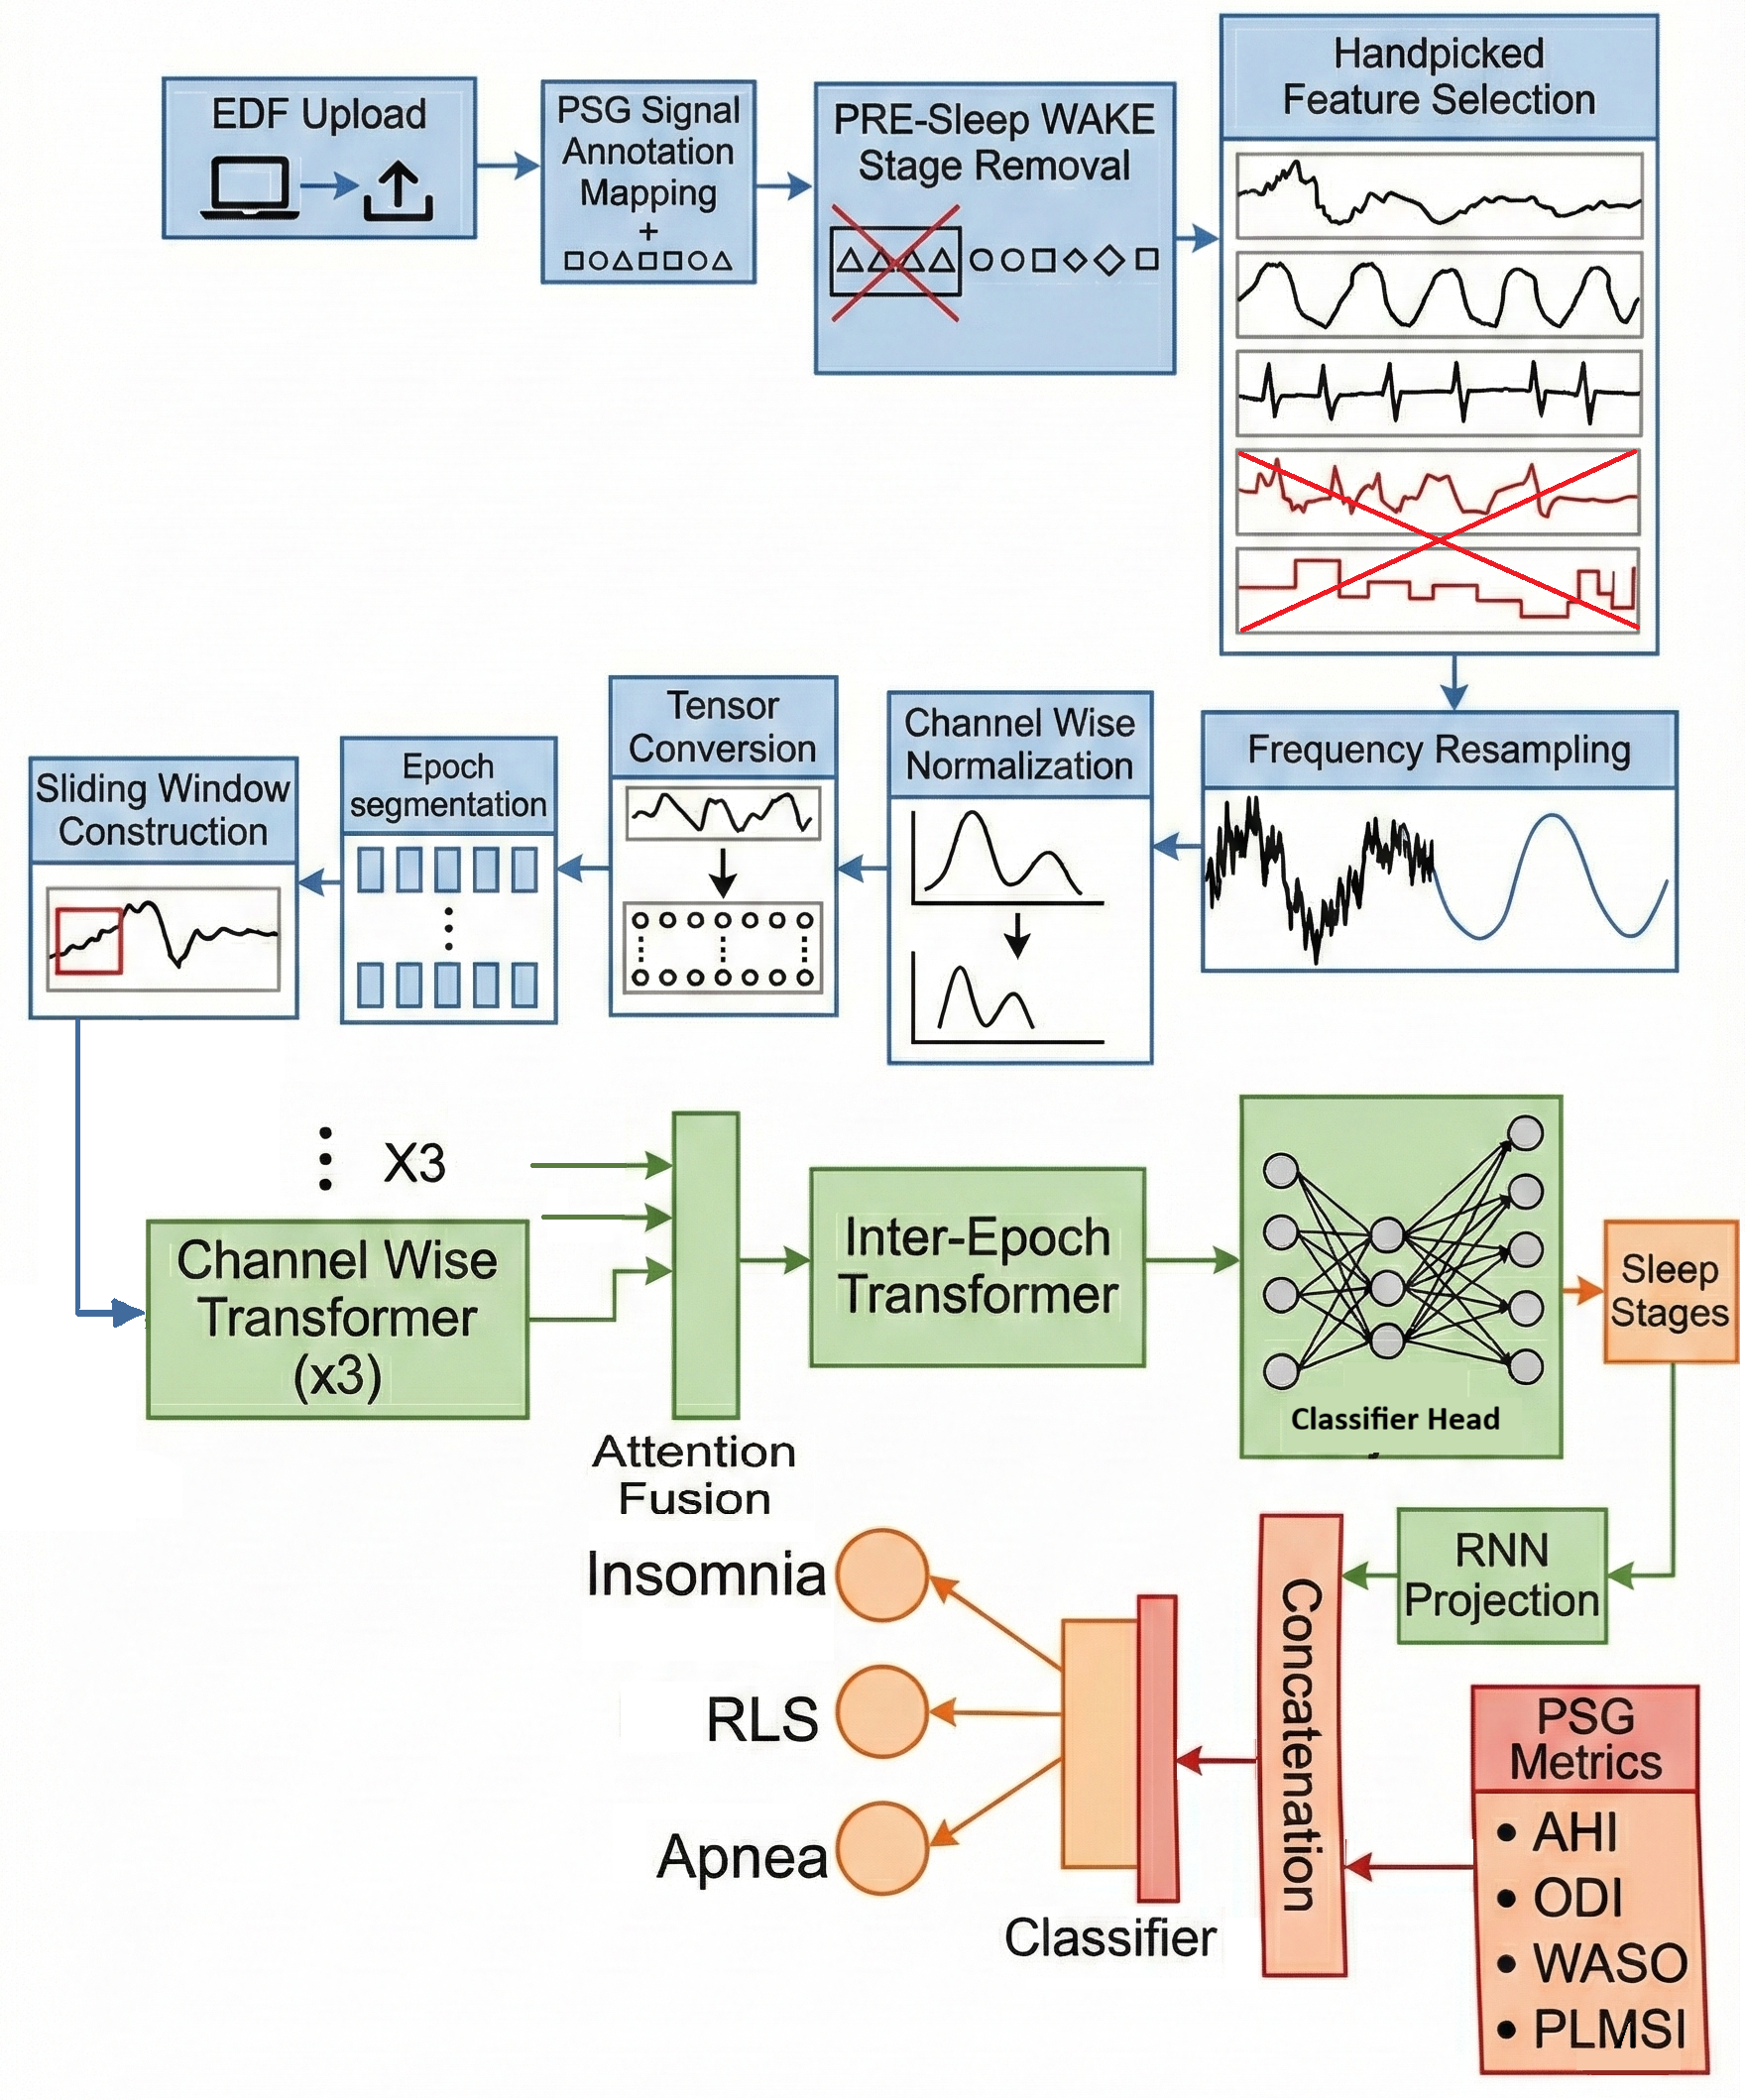
\includegraphics[width=\linewidth]{DFD_P2.png}
    \caption{Data Flow Diagram Level 2 - End-To-End Data Flow Pipeline from PSG signal reading to Disorder detection.}
    \label{fig:transformer_arch}
\end{figure}

The dataset provides a wide range of physiological channels sampled at different frequencies. EEG channels are recorded at 256~Hz, including Fz--Cz, Oz--Cz, and C4--M1 derivations, along with their corresponding offset signals. Additional modalities include electrooculography channels sampled at 256~Hz, electrocardiography at 256~Hz, electromyography at 256~Hz, respiratory and airflow signals sampled at 32~Hz, plethysmography and oxygen saturation signals at 32~Hz, heart rate and oxygen status signals at 1~Hz, and auxiliary sensors such as body position, snoring, abdominal effort, and thermal airflow. While the dataset supports multimodal analysis, this work intentionally focuses on EEG signals to isolate neural activity patterns that are directly responsible for sleep stage discrimination.



\subsubsection{EEG Channel Selection}

Three EEG derivations were selected for modeling: Fz--Cz, Oz--Cz, and C4--M1. This selection reflects a deliberate balance between neurophysiological coverage and computational efficiency. The Fz--Cz channel captures frontal-central activity, which is strongly associated with sleep onset dynamics, slow eye movements, and hallmark features of light sleep such as K-complexes and sleep spindles. The Oz--Cz derivation emphasizes occipital activity and provides sensitivity to alpha rhythms that dominate wakefulness and diminish during the transition to sleep, as well as patterns relevant to REM sleep. The C4--M1 channel, positioned over the central cortex, is particularly informative for detecting delta oscillations and high-amplitude slow waves that characterize deep sleep stages such as N3 and N4.

By combining frontal, occipital, and central perspectives, the selected channels provide complementary views of brain activity that collectively encode the defining characteristics of all major sleep stages. Restricting the input to three EEG channels reduces redundancy, limits overfitting, and enables the model to focus on the most diagnostically relevant neural signals, following the principle of minimal channel selection demonstrated in prior work~\cite{wadichar2023two,wilaiprasitporn2017hypnodensity}.

\subsubsection{Signal Conditioning and Temporal Alignment}

Raw EEG recordings exhibit substantial inter-subject variability, baseline drift, and noise introduced by electrode placement and recording conditions. Moreover, recordings often begin with extended wake periods that contribute disproportionately to class imbalance and introduce non-sleep artifacts. To mitigate these issues, a structured offline preprocessing pipeline was employed.

All EEG channels were resampled to a uniform sampling rate of 128~Hz to ensure temporal alignment and reduce computational overhead while preserving sufficient spectral resolution for sleep-related oscillations. The initial continuous wake segment, identified using hypnogram annotations, was removed to reduce class imbalance and eliminate artifacts commonly present at the beginning of recordings. Channel-wise z-score normalization was applied to standardize signal distributions across subjects, improving numerical stability and facilitating effective gradient-based optimization during training.

\subsubsection{Epoch Segmentation and Tensor Representation}

Following preprocessing, each recording was segmented into non-overlapping 30-second epochs, consistent with clinical sleep staging standards. At a sampling rate of 128~Hz, each epoch contains 3840 time samples per channel. The processed EEG signals were stored as fixed-shape tensors of dimension $(3, T)$, where the three channels correspond to Fz--Cz, Oz--Cz, and C4--M1, and $T$ denotes the total number of samples after trimming and resampling.

Converting the data into tensor files offers several advantages over direct EDF-based processing. Tensor representations enable efficient memory-mapped loading, deterministic indexing, and seamless integration with deep learning frameworks. This design choice significantly reduces input-output overhead during training and ensures that preprocessing decisions are fixed and reproducible across experiments.

\subsection{Sequence Construction and Temporal Context Modeling}

Sleep stages are temporally correlated, and an epoch's label often depends on preceding and succeeding epochs. To explicitly model this dependency, the dataset was organized into sequences using a sliding window approach. Each sample consists of a sequence of 20 consecutive epochs, corresponding to approximately ten minutes of sleep. A stride of one epoch was used to maximize data utilization while preserving temporal continuity. Sequences containing unscored or invalid epochs were excluded to ensure reliable supervision.

This formulation enables the model to learn both short-term transitions, such as wake-to-N1 shifts, and long-term structural patterns, such as progression into deep sleep and REM cycles, which are essential for physiologically consistent sleep staging.

\subsection{Hierarchical Model Architecture}

\subsubsection{Epoch-Level Feature Extraction}

Within each epoch, EEG channels are processed independently using one-dimensional convolutional networks. This stage addresses the challenge of extracting meaningful representations from high-resolution raw signals. Convolutional filters act as learnable temporal feature extractors, capturing frequency-specific patterns associated with sleep phenomena such as spindles, alpha rhythms, and slow waves. Pooling operations progressively reduce temporal resolution, producing compact token sequences that summarize intra-epoch dynamics while retaining sensitivity to transient events.

\subsubsection{Challenges in Raw Signal Representation Learning}

Early experiments revealed that directly feeding raw EEG signals into attention-based architectures resulted in unstable training and excessive memory consumption due to the high temporal resolution of the data. Additionally, Transformers operating directly on raw time-series tokens struggled to learn meaningful representations without strong inductive biases, often attending to noise rather than physiologically relevant patterns.

To address this, convolutional layers were introduced as a front-end feature extractor. These layers act as learnable temporal filters that mimic classical signal processing operations such as band-pass filtering, while allowing end-to-end optimization. Pooling operations were incorporated to reduce temporal dimensionality and computational cost, enabling the downstream Transformer modules to focus on semantically meaningful temporal summaries rather than raw sample-level fluctuations. This design significantly stabilized training and improved convergence speed across experiments.

\subsubsection{Intra-Epoch Temporal Attention}

While convolutional layers capture local temporal patterns, they are limited in modeling long-range dependencies within an epoch. To overcome this limitation, the convolutional tokens for each channel are passed through a Transformer encoder equipped with positional encoding. Self-attention allows the model to selectively emphasize salient temporal segments, regardless of their absolute position within the epoch, thereby improving robustness to temporal variability and enhancing representational expressiveness.

\begin{figure}[htbp]
    \centering
    \includegraphics[width=\linewidth]{transformer_Arch_cropped.pdf}
    \caption{Custom Hierarchial Transformer modelling both global inter-epoch embeddings and local inter-channel embeddings.}
    \label{fig:transformer_arch}
\end{figure}

\subsubsection{Empirical Evaluation of Temporal Modeling Within Epochs}

Although convolutional networks capture local temporal patterns effectively, experiments without explicit attention mechanisms demonstrated limited sensitivity to long-duration EEG events such as extended spindle activity or slow-wave complexes spanning several seconds. Fixed receptive fields constrained the model’s ability to adaptively focus on temporally salient regions.

\begin{table*}[!t]
\centering
\renewcommand{\arraystretch}{1.25}
\begin{tabular}{|p{4.5cm}|p{5.8cm}|p{6.2cm}|}
\hline
\textbf{Feature Name} & \textbf{Physiological Meaning} & \textbf{Clinical Insight} \\
\hline

Apnea--Hypopnea Index (AHI, 3\% desaturation or arousal) &
Measures the average number of apnea and hypopnea events per hour of sleep, defined by respiratory pauses accompanied by oxygen desaturation or EEG arousals. &
Primary marker for obstructive sleep apnea severity. Elevated values indicate frequent airway obstruction, intermittent hypoxia, and repeated sleep fragmentation, which are linked to cardiovascular and metabolic complications. \\
\hline

Total Arousal Index &
Quantifies the frequency of brief cortical arousals per hour of sleep, regardless of underlying cause. &
Reflects global sleep fragmentation. Increased arousal frequency is commonly observed in insomnia, sleep apnea, and movement-related sleep disorders, contributing to non-restorative sleep and daytime impairment. \\
\hline

Oxygen Desaturation Index (3\%) &
Counts the number of oxygen saturation drops of at least 3\% per hour of sleep. &
Provides a direct measure of nocturnal hypoxemia and respiratory instability. Particularly informative for identifying sleep apnea and assessing its physiological impact beyond event counts alone. \\
\hline

Percentage of Sleep Time in Stage N1 &
Represents the proportion of total sleep spent in light transitional sleep. &
Elevated N1 duration indicates unstable or superficial sleep and is frequently associated with insomnia and sleep apnea, where frequent arousals prevent progression into deeper sleep stages. \\
\hline

Percentage of Sleep Time in Stage N2 &
Represents the proportion of total sleep spent in intermediate non-REM sleep. &
Alterations in N2 duration may indicate disrupted sleep architecture. Reduced N2 continuity is often linked to sleep fragmentation, while excessive N2 may compensate for reduced deep sleep in disordered conditions. \\
\hline

Percentage of Sleep Time in Deep Sleep (N3/N4) &
Measures the proportion of slow-wave sleep associated with physical restoration and metabolic regulation. &
Reduced deep sleep is a hallmark of insomnia and sleep apnea. Loss of slow-wave sleep is linked to impaired recovery, cognitive dysfunction, and increased cardiometabolic risk. \\
\hline

Percentage of Sleep Time in REM Sleep &
Represents the proportion of sleep spent in rapid eye movement sleep, associated with dreaming and memory consolidation. &
Abnormal REM proportions suggest REM instability. Reduced REM is common in sleep apnea due to frequent arousals, while altered REM patterns may also indicate parasomnias or narcolepsy-related abnormalities. \\
\hline

Sleep Efficiency &
Ratio of total sleep time to total time spent in bed. &
A global indicator of sleep quality. Low sleep efficiency is a core diagnostic feature of insomnia and reflects prolonged sleep latency, frequent awakenings, or early morning awakenings. \\
\hline

Wake After Sleep Onset (WASO) &
Total duration of wakefulness occurring after initial sleep onset. &
High WASO is strongly associated with sleep maintenance insomnia and fragmented sleep caused by apnea or periodic limb movements, leading to poor sleep continuity. \\
\hline

Periodic Limb Movement Arousal Index &
Frequency of limb movements during sleep that are associated with cortical arousals. &
Key indicator of periodic limb movement disorder and restless legs syndrome. Elevated values reflect movement-induced sleep disruption and recurrent micro-arousals. \\
\hline

Sleep Period Duration &
Elapsed time between sleep onset and final awakening. &
Abnormal sleep period duration may indicate circadian rhythm disturbances, insomnia, or poor sleep consolidation resulting from frequent awakenings or early termination of sleep. \\
\hline

REM-Related Limb Movement Arousal Index &
Measures limb movements associated with arousals occurring specifically during REM sleep. &
Provides insight into REM sleep instability and REM-related movement disorders. Elevated values may suggest REM sleep behavior disorder or REM-specific motor dysregulation. \\
\hline

\end{tabular}
\caption{Description of polysomnography-derived features and their clinical relevance for sleep disorder detection}
\label{tab:psg_features}
\end{table*}


The introduction of Transformer-based self-attention within each epoch allowed the model to dynamically reweight temporal segments based on contextual relevance. Positional encoding was incorporated to preserve temporal ordering, which was found to be critical for maintaining physiological interpretability. Ablation experiments confirmed that removing intra-epoch attention resulted in degraded performance for stages characterized by transient or sparse EEG features, particularly N1 and REM, validating the necessity of this component.


\subsubsection{Channel-Wise Attention Fusion}

The relative importance of EEG channels varies across sleep stages and individuals. To accommodate this variability, channel-specific representations are fused using a channel-wise attention mechanism. This component enables the model to dynamically weight information from Fz--Cz, Oz--Cz, and C4--M1 based on their relevance to the current epoch, addressing spatial heterogeneity without imposing fixed channel importance.

\begin{figure*}
	\centerline{\includegraphics[scale=0.32]{Methodology_p2.png}}
	\caption{Methodology Pipeline}
	\label{methodology}
\end{figure*}

The fused epoch embeddings are processed by a second Transformer encoder operating across the sequence dimension. This inter-epoch module captures long-range temporal dependencies and enforces contextual consistency across predictions. By attending over neighboring epochs, the model learns structured sleep architecture patterns, such as stage persistence and cyclic progression, which are difficult to encode using isolated epoch-level models.

\subsubsection{Capturing Sleep Architecture and Long-Range Dependencies}

A critical limitation observed in epoch-wise and shallow sequence models was their inability to enforce global sleep architecture constraints. Models trained without explicit inter-epoch context frequently produced physiologically implausible stage transitions, such as abrupt shifts from deep sleep to wakefulness without intermediate stages.

The inter-epoch Transformer was introduced to explicitly model long-range dependencies across sequences of epochs. By attending across the temporal dimension, this module learns patterns such as stage persistence, gradual transitions, and cyclic sleep organization. Experiments confirmed that this component significantly reduced prediction fragmentation and improved consistency across entire sleep episodes, leading to higher macro-level performance metrics.

\subsubsection{Addressing Spatial Variability and Channel Dominance}

Initial fusion strategies based on simple concatenation or averaging of channel representations implicitly assumed equal importance across EEG channels. However, empirical analysis of attention maps and intermediate activations revealed that different sleep stages rely disproportionately on specific cortical regions. For example, frontal-central activity dominated during light sleep transitions, whereas central derivations were more informative during deep sleep.

Channel-wise attention was therefore introduced to allow the model to learn adaptive, data-driven weighting of EEG channels. This mechanism mitigates the risk of channel dominance bias and improves robustness to inter-subject variability. Comparative experiments demonstrated that attention-based fusion consistently outperformed static fusion strategies, particularly in subjects with atypical EEG patterns or reduced signal quality in specific channels.

\subsubsection{Classification Layer}

Finally, a fully connected classification head maps each context-aware epoch embedding to sleep stage logits. Predictions are generated for all epochs within a sequence simultaneously, enabling end-to-end sequence-to-sequence learning. This formulation ensures that each epoch’s classification is informed by both its internal EEG structure and its surrounding temporal context.


\subsection{Experimental Motivation for Hierarchical Design}

During preliminary experimentation, several baseline architectures were evaluated to assess their suitability for sleep stage classification. Initial experiments using purely convolutional models operating on individual epochs demonstrated reasonable performance for dominant stages such as Wake and N2 but suffered from poor discrimination of transitional and minority stages, particularly N1 and REM. These models exhibited fragmented predictions and failed to maintain temporal consistency across consecutive epochs.

Subsequently, recurrent neural networks operating on handcrafted spectral features were explored to introduce temporal context. While recurrent models improved continuity, their reliance on fixed feature representations limited their ability to capture fine-grained EEG microstructures, and performance degraded as sequence length increased. These observations highlighted the necessity of a hierarchical approach that combines local signal-level feature extraction with global temporal modeling. The final architecture therefore integrates convolutional encoders for low-level EEG representation learning and Transformer-based attention mechanisms for modeling both intra-epoch and inter-epoch dependencies.


\subsection{Training Strategy}

The model is trained using categorical cross-entropy loss computed across all epochs in each sequence. Gradient clipping is applied to stabilize optimization in deep attention-based architectures. The dataset is partitioned into training, validation, and test splits at the sequence level to prevent temporal leakage and ensure unbiased evaluation.

\subsection{Optimization Challenges and Stability Considerations}

\begin{figure*}
	\centerline{\includegraphics[scale=0.40]{per_class_metrics.png}}
	\caption{Per Class Metrics Curve: F1 Score vs Epochs (Top Left), Precision vs Epocs (Top Right), Recall vs Epochs (Bottom Left), ROC AUC vs Epoch (Bottom Right)}
	\label{methodology}
\end{figure*}

Training deep attention-based architectures on EEG data posed several optimization challenges. Early experiments exhibited unstable gradients and slow convergence, particularly when long sequences were used. Gradient clipping was therefore employed to prevent exploding gradients, which proved essential for stable training across multiple random initializations.


Additionally, standard accuracy-based evaluation was found to be misleading due to the class imbalance inherent in sleep staging data, where certain stages dominate the distribution. Consequently, training and validation monitoring emphasized class-sensitive metrics, including per-class recall and macro-averaged performance measures. This shift in evaluation strategy ensured that improvements reflected genuine gains in minority stage discrimination rather than trivial majority-class dominance.

\begin{table*}[t]
\centering
\renewcommand{\arraystretch}{1.4}
\begin{tabular}{|c|cccccc|}
\hline
\multirow{\textbf{True Stage}} & 
\multicolumn{6}{c|}{\textbf{Predicted Stage}} \\ \cline{2-7}

& \textbf{W} & \textbf{N1} & \textbf{N2} & \textbf{N3} & \textbf{N4} & \textbf{REM} \\ \hline

\textbf{W}   
& 3764 & 1121 & 115 & 124 & 0 & 491 \\ \hline

\textbf{N1}  
& 155 & 640 & 140 & 110 & 0 & 228 \\ \hline

\textbf{N2}  
& 281 & 913 & 1048 & 2600 & 0 & 643 \\ \hline

\textbf{N3}  
& 9 & 6 & 26 & 900 & 0 & 37 \\ \hline

\textbf{N4}  
& 0 & 0 & 0 & 0 & 0 & 0 \\ \hline

\textbf{REM} 
& 220 & 472 & 151 & 63 & 0 & 743 \\ \hline

\end{tabular}
\caption{Confusion matrix for sleep stage classification on the test set. Rows denote true sleep stages and columns denote predicted sleep stages.}
\label{tab:confusion_matrix_test_set}
\end{table*}

\subsection{Experimental Baselines and Model Validation}

To contextualize the effectiveness of the proposed architecture, multiple baseline models were evaluated during development, including traditional machine learning classifiers trained on handcrafted sequence features and simplified neural architectures with reduced temporal modeling capacity. These baselines consistently underperformed the proposed hierarchical Transformer, particularly in capturing transitional sleep stages and maintaining temporal coherence.

Comparative analysis across these experiments informed architectural refinements and confirmed that the combination of convolutional feature extraction, intra-epoch attention, channel-wise fusion, and inter-epoch context modeling is necessary to achieve robust and physiologically consistent sleep stage classification.

\section{Performance Evaluation}
\label{sec:results}

This section presents a comprehensive evaluation of the proposed transformer-based sleep staging model and the downstream sleep disorder classification framework. The analysis integrates quantitative performance assessment with qualitative interpretation to understand model behaviour, error characteristics, and clinical relevance.


\subsection{Experimental Setup}

The proposed system was evaluated on held-out validation and test sets constructed from full-night polysomnography (PSG) recordings. Multichannel physiological signals were segmented into fixed-length epochs following standard sleep scoring guidelines and provided as input to the transformer-based sleep staging model. The model predicts six sleep stages: Wake (W), N1, N2, N3, N4, and REM.

Predicted sleep stages were subsequently used to derive clinically relevant sleep metrics, including stage proportions, sleep continuity indicators, and transition-based features. These aggregated metrics served as input to a lightweight classifier designed to detect insomnia, restless leg disorder, and obstructive sleep apnea. Sleep staging and disorder detection were evaluated independently to analyse error propagation across the pipeline.

\subsection{Evaluation Metrics Used}

Sleep stage classification performance was assessed using overall accuracy, class-wise precision, recall, and F1-score. Normalized confusion matrices were employed to examine inter-stage confusion patterns. Both macro-averaged and weighted metrics were reported to account for significant class imbalance across sleep stages.

For disorder classification, receiver operating characteristic (ROC) curves and area under the ROC curve (ROC--AUC) were used to evaluate discriminative capability. Precision--recall (PR) curves and average precision (AP) scores were additionally computed, as PR analysis provides a more informative evaluation under imbalanced class distributions.

\begin{table}[t]
\centering
\renewcommand{\arraystretch}{1.7}
\begin{tabular}{|c|c|c|c|}
\hline
\textbf{Sleep Stage} & \textbf{Precision} & \textbf{Recall} & \textbf{F1-Score} \\ \hline

W   & 0.84 & 0.71 & 0.77 \\ \hline
N1  & 0.20 & 0.49 & 0.29 \\ \hline
N2  & 0.74 & 0.20 & 0.31 \\ \hline
N3  & 0.25 & 0.91 & 0.39 \\ \hline
N4  & 0.00 & 0.00 & 0.00 \\ \hline
REM & 0.33 & 0.42 & 0.37 \\ \hline

\end{tabular}
\caption{Per-class precision, recall, and F1-score for sleep stage classification on the validation set.}
\label{tab:per_class_metrics_validation}
\end{table}
\begin{table}[t]
\centering
\renewcommand{\arraystretch}{2}
\begin{tabular}{|l|c|}
\hline
\textbf{Metric} & \textbf{Score} \\ \hline

Overall Accuracy   & 0.491 \\ \hline
Macro Precision    & 0.392 \\ \hline
Macro Recall       & 0.454 \\ \hline
Macro F1-score     & 0.354 \\ \hline
Weighted Precision & 0.653 \\ \hline
Weighted Recall    & 0.491 \\ \hline
Weighted F1-score  & 0.500 \\ \hline

\end{tabular}
\caption{Overall and averaged performance metrics for sleep stage classification on the validation set.}
\label{tab:summary_metrics_validation}
\end{table}



\subsection{Quantitative Results}

The transformer-based sleep staging model achieved an overall validation accuracy of approximately 49\%, with a macro F1-score of 0.35 and a weighted F1-score of 0.50. Class-wise analysis revealed substantial variation in performance across sleep stages. Deep sleep (N3) was classified with high reliability, achieving a true positive rate of approximately 92\%. This result reflects the strong spectral and temporal characteristics of slow-wave activity, which are effectively captured by the attention mechanism.



Wake and REM sleep were classified with moderate accuracy, achieving correct prediction rates of 67\% and 45\%, respectively. Frequent confusion was observed between REM and N1, consistent with their shared low-amplitude EEG characteristics and transitional dynamics. Light sleep stages N1 and N2 exhibited the lowest recall and precision, with N1 often misclassified as wakefulness and N2 confused with N3 or REM. The absence of N4 samples in the test set further exacerbated class imbalance and indirectly influenced neighbouring stage predictions.



At the disorder level, the classifier achieved ROC--AUC values of 0.568 for insomnia, 0.540 for restless leg disorder, and 0.614 for sleep apnea. Precision--recall analysis indicated low average precision across all disorders, with sleep apnea demonstrating comparatively higher precision at low recall levels. These results suggest modest but meaningful discriminative capability, particularly for disorders associated with global sleep architecture disruption.

\subsection{Comparison with Baselines or Related Work}

The observed sleep staging performance is consistent with prior deep learning–based approaches~\cite{xu2022deep,wadichar2023two}, which similarly report strong recognition of stable sleep stages such as N3 and Wake, alongside persistent difficulty in discriminating light sleep stages. Transformer-based architectures have been shown to outperform conventional convolutional and recurrent models in capturing long-range temporal dependencies~\cite{chen2022joint}; however, light sleep ambiguity remains a common limitation across studies.

For disorder detection, the achieved ROC--AUC values are comparable to existing PSG-based screening systems that rely primarily on sleep stage distributions and summary statistics~\cite{xu2022deep,alattar2024cap}. Studies that report higher apnea detection performance typically incorporate explicit respiratory event modelling or oxygen desaturation indices~\cite{wongsirichot2017minimal}. In contrast, the proposed framework maintains competitive discrimination using only derived sleep metrics, favouring computational efficiency and scalability.

Unlike many existing works that focus exclusively on diagnosis~\cite{xu2022deep,urtnasan2021sleep,urtnasan2022plmd}, the proposed system uniquely integrates explainable artificial intelligence modules and patient-facing guidance mechanisms, which are generally absent in baseline approaches~\cite{aziz2025wearable}.

\section{Discussion}

The experimental results highlight several important observations regarding model behaviour and system-level performance. The strong classification of N3 confirms the transformer's effectiveness in modelling long-range temporal patterns and stable physiological signatures~\cite{chen2022joint}. In contrast, reduced performance on N1 and N2 reflects the inherent ambiguity of transitional sleep and sensitivity to channel selection and signal quality, consistent with findings in single-channel EEG approaches~\cite{wadichar2023two}.

At the disorder level, conditions characterised by global sleep fragmentation, such as obstructive sleep apnea, are more robust to staging errors, as their diagnostic signatures emerge from aggregate sleep disruption rather than precise stage boundaries~\cite{alattar2024cap}. Conversely, insomnia and restless leg disorder depend on subtle transitions and episodic micro-arousals~\cite{urtnasan2022plmd,umut2016plm}, making their detection more susceptible to error propagation from the sleep staging module.

The disparity between macro-averaged and weighted metrics further underscores the impact of class imbalance, with dominant stages and disorders disproportionately influencing overall performance. Despite moderate quantitative accuracy, the inclusion of explainable outputs enables clinically meaningful interpretation of predictions, supporting transparent decision-making.

Overall, the results demonstrate the feasibility of transformer-based PSG analysis for automated sleep staging and preliminary disorder screening, while highlighting the need for improved light sleep modelling, event-level feature integration, and enhanced imbalance handling to achieve clinically robust performance.

% Experimental Setup

% Evaluation Metrics Used

% Quantitative Results

% Comparison with Baselines or Related Work

% Discussion

\section{CONCLUSIONS}
\label{sec:conclusion}

This work addressed the challenge of scalable, interpretable, and accessible sleep disorder detection using polysomnography data, with particular emphasis on overcoming the limitations of conventional in-laboratory diagnosis and black-box artificial intelligence systems. The primary objective was to develop an automated framework capable of reliable sleep stage classification, clinically meaningful disorder inference, and patient-centric guidance, while remaining suitable for deployment in resource-constrained settings.

To achieve this goal, a transformer-based sleep staging architecture was designed to model long-range temporal dependencies in multichannel EEG signals, followed by extraction of clinically grounded sleep metrics for downstream disorder classification. The framework integrates explainable artificial intelligence techniques to provide interpretable visualizations and structured clinical insights, alongside a retrieval-augmented generation mechanism that delivers personalized medical explanations and lifestyle recommendations. The unified integration of automated sleep staging, interpretable disorder detection, and patient-facing guidance within a single web-based platform distinguishes this work from prior approaches that treat diagnosis, explanation, and user interaction as independent components.

Experimental evaluation on the MESA sleep dataset demonstrated that the proposed transformer model effectively captures stable sleep stages such as deep sleep, achieving recall exceeding 90\%, while the disorder classifier exhibits meaningful discriminative capability across multiple conditions. At the same time, the analysis revealed persistent challenges in discriminating light sleep stages, particularly N1 and N2, which exhibited lower precision and recall. These findings reflect the inherent ambiguity of transitional sleep states and their sensitivity to signal quality and inter-subject variability, consistent with trends reported in manual scoring agreement studies.

Beyond quantitative performance, the system emphasizes transparency, accessibility, and user engagement. By combining automated analysis with clinically interpretable outputs and interactive patient education, the proposed solution supports early screening, improves sleep health awareness, and facilitates scalable deployment in low-resource environments. The framework is designed to bridge the gap between clinical expertise and public usability, offering a transparent and privacy-conscious approach to sleep disorder assessment and management.

Despite these contributions, several limitations warrant consideration. The moderate performance on light sleep stages and the limited accuracy of disorder classification indicate that the system currently functions as a decision support tool rather than an autonomous diagnostic solution. The exclusive reliance on EEG signals, while enhancing accessibility, omits complementary diagnostic information from respiratory, cardiac, and electromyographic modalities. In addition, the absence of explicit event-level detection for apneas, arousals, and limb movements constrains disorder characterization. Evaluation on a single dataset further limits conclusions regarding generalizability, and the patient-facing guidance components have not yet undergone clinical or user-centered validation.

\subsection{Future Directions}

Future research will focus on extending the current framework to address these limitations while enhancing clinical utility and real-world impact. A key direction involves the integration of multimodal PSG signals, including respiratory, oxygen saturation, ECG, and EMG channels, using interpretable fusion mechanisms that preserve transparency while improving robustness. Incorporating explicit event detection modules for respiratory and movement-related events would enable direct computation of standard clinical indices and support severity stratification. Joint optimization of sleep staging and event detection through multi-task learning may further improve performance consistency across sleep stages and disorders.

Additional efforts will explore advanced strategies for mitigating class imbalance and inter-subject variability, including cost-sensitive learning, generative augmentation, and architecture-level adaptations tailored to minority classes. Validation across multiple independent datasets representing diverse populations and recording conditions is essential to establish generalizability. Privacy-preserving training paradigms such as federated learning can facilitate collaborative model development across institutions without centralized data sharing, while model compression and optimization techniques can enable deployment on edge and low-resource devices.

Equally important are future enhancements to user interaction and clinical integration. Longitudinal analysis across multiple nights may support trend-based risk assessment, while deeper incorporation of lifestyle and behavioral data can enable adaptive, personalized recommendations. Prospective clinical studies and user-centered evaluations are required to assess usability, trust, and impact on outcomes such as time-to-diagnosis, treatment adherence, and quality of life.

The deployment of automated sleep analysis systems also raises ethical considerations that must be addressed alongside technical advancement. Ensuring data privacy, minimizing algorithmic bias, supporting clinical autonomy, and promoting equitable access are essential for responsible adoption. The system should remain explicitly positioned as a clinical decision support tool requiring human oversight rather than a replacement for expert judgment.

In conclusion, this work demonstrates the feasibility of an integrated framework combining transformer-based sleep staging, interpretable disorder detection, and patient-centric guidance for advancing accessible sleep health assessment. While significant progress has been achieved, continued methodological refinement, broader validation, and responsible deployment are necessary to realize the full potential of such systems. Ultimately, the success of automated sleep disorder screening technologies will be measured by their ability to improve healthcare accessibility, support clinical decision-making, and reduce the substantial burden of undiagnosed and undertreated sleep disorders.

% 1. Restate the problem and goal

% Briefly remind the reader what you set out to solve.

% 2. Summarize the methodology and what you achieved

% One or two sentences on the approach and main results.

% 3. Highlight the key findings or contributions

% What is the main takeaway of your work?

% 4. Mention limitations and future work

% What could be improved? What can be explored next?
 

% \addtolength{\textheight}{-12cm}   % This command serves to balance the column lengths
                                  % on the last page of the document manually. It shortens
                                  % the textheight of the last page by a suitable amount.
                                  % This command does not take effect until the next page
                                  % so it should come on the page before the last. Make
                                  % sure that you do not shorten the textheight too much.

%%%%%%%%%%%%%%%%%%%%%%%%%%%%%%%%%%%%%%%%%%%%%%%%%%%%%%%%%%%%%%%%%%%%%%%%%%%%%%%%



%%%%%%%%%%%%%%%%%%%%%%%%%%%%%%%%%%%%%%%%%%%%%%%%%%%%%%%%%%%%%%%%%%%%%%%%%%%%%%%%



%%%%%%%%%%%%%%%%%%%%%%%%%%%%%%%%%%%%%%%%%%%%%%%%%%%%%%%%%%%%%%%%%%%%%%%%%%%%%%%%
% \section*{APPENDIX}

% Software and Environment Setup\\

% Training Procedure Code (Simplified) - 
% Add clean code snippets, not the entire program \\
\section*{APPENDIX}

\subsection{Software and Hardware Environment}

All experiments were conducted on a local workstation configured with Windows~11 (64-bit), equipped with an Intel Core i7 (12th Generation) CPU, 64~GB system memory, and an NVIDIA T400 GPU. The hardware configuration reflects a mid-range computational setup, chosen deliberately to evaluate the feasibility of training and deploying the proposed models on resource-constrained systems rather than high-end compute servers.

Model development and training were implemented using the PyTorch deep learning framework, enabling flexible definition of custom architectures, loss functions, and training schedules. Annotation files provided in XML format were parsed using Python’s built-in \texttt{xml} library, while raw polysomnography recordings stored in EDF format were processed using the \texttt{mne} library. Additional system utilities such as \texttt{argparse}, \texttt{glob}, \texttt{os}, \texttt{warnings}, \texttt{numpy}, and \texttt{math} were used for configuration management, file handling, numerical operations, and runtime control.

To reduce runtime memory consumption and input--output overhead during training, all PSG signals were preprocessed offline and stored as serialized tensor files. This design choice ensured deterministic data access, minimized repeated EDF parsing, and enabled efficient batching during training.

\subsection{Memory Management and Runtime Stability Measures}

Given the limited GPU memory available, several safeguards were incorporated to prevent memory fragmentation and training instability. Intermediate tensors were explicitly dereferenced after use, and Python’s garbage collection module was periodically invoked to free unused memory. Additionally, GPU memory usage was monitored and controlled to avoid excessive allocation during long training runs.

\begin{lstlisting}[language=Python]
import gc
import torch

# Periodic memory cleanup during training
torch.cuda.empty_cache()
gc.collect()
\end{lstlisting}

These measures allowed stable training of attention-based sequence models even under constrained GPU resources.

\subsection{Training Procedure Overview}

Training was performed using sequence-level supervision, where each sample consisted of multiple consecutive sleep epochs. To address severe class imbalance inherent in sleep stage distributions, focal loss with class-dependent weighting was employed. Gradient clipping was applied to stabilize optimization in deep Transformer architectures, and cosine annealing was used for adaptive learning rate scheduling.

\begin{lstlisting}[language=Python]
# Forward pass
output = model(features)
logits = output['logits']  # (batch, seq_len, num_classes)

# Flatten predictions and labels
logits_flat = logits.view(-1, num_classes)
labels_flat = labels.view(-1)

# Compute focal loss
loss = criterion(logits_flat, labels_flat)

# Backpropagation with gradient clipping
loss.backward()
torch.nn.utils.clip_grad_norm_(model.parameters(), max_norm=1.0)
optimizer.step()
\end{lstlisting}

This procedure ensured that difficult-to-classify stages such as N1 and transitional epochs contributed more strongly to parameter updates.

\subsection{Class Weight Estimation for Imbalanced Data}

Class weights were computed dynamically from the training data to reduce bias toward dominant sleep stages. A square-root inverse frequency strategy was adopted to balance stability and sensitivity, avoiding excessively large weights for rare classes.

\begin{lstlisting}[language=Python]
# Compute class weights
class_counts = torch.clamp(class_counts, min=1.0)
total_samples = class_counts.sum()

class_weights = torch.sqrt(total_samples / class_counts)
class_weights = class_weights / class_weights.mean()
\end{lstlisting}

These weights were incorporated directly into the focal loss formulation, improving macro-averaged performance without destabilizing training.

\subsection{Validation, Model Selection, and Checkpointing}

Model selection was based on macro-averaged F1-score rather than overall accuracy, ensuring balanced performance across sleep stages. Checkpoints were saved whenever an improvement in validation macro F1-score was observed, enabling recovery from interruptions and preventing overfitting.

\begin{lstlisting}[language=Python]
if val_f1_macro > best_val_f1:
    best_val_f1 = val_f1_macro
    torch.save({
        'epoch': epoch,
        'model_state_dict': model.state_dict(),
        'optimizer_state_dict': optimizer.state_dict(),
        'scheduler_state_dict': scheduler.state_dict()
    }, checkpoint_path)
\end{lstlisting}

This strategy prioritizes physiologically meaningful performance improvements over trivial gains driven by majority classes.

\subsection{Baseline Machine Learning Comparisons}

In addition to the proposed deep learning models, traditional machine learning classifiers including Support Vector Machines, Random Forests, and Gradient Boosted Trees were trained using engineered sequence-level features. Stratified sampling and threshold optimization were applied to ensure fair comparison under class imbalance.

\begin{lstlisting}[language=Python]
# Optimize decision thresholds to maximize F1-score
def score_func(threshold):
    preds = (probs >= threshold).astype(int)
    return -f1_score(y_true, preds)

optimal_threshold = minimize_scalar(
    score_func, bounds=(0.0, 1.0), method='bounded'
).x
\end{lstlisting}

These baselines provide a reference point for evaluating the advantages of end-to-end temporal modeling over static feature-based approaches.

\subsection{Reproducibility Considerations}

All experiments were conducted with fixed random seeds for dataset splitting, weight initialization, and optimizer behavior. Configuration parameters were exposed through command-line arguments, and intermediate artifacts such as dataset splits, checkpoints, and evaluation outputs were stored for traceability and reproducibility.

---





%%%%%%%%%%%%%%%%%%%%%%%%%%%%%%%%%%%%%%%%%%%%%%%%%%%%%%%%%%%%%%%%%%%%%%%%%%%%%%%%

\bibliographystyle{unsrt}
\bibliography{bibil.bib}



\end{document}
